% The document class supplies options to control rendering of some standard
% features in the result.  The goal is for uniform style, so some attention 
% to detail is *vital* with all fields.  Each field (i.e., text inside the
% curly braces below, so the MEng text inside {MEng} for instance) should 
% take into account the following:
%
% - author name       should be formatted as "FirstName LastName"
%   (not "Initial LastName" for example),
% - supervisor name   should be formatted as "Title FirstName LastName"
%   (where Title is "Dr." or "Prof." for example),
% - degree programme  should be "BSc", "MEng", "MSci", "MSc" or "PhD",
% - dissertation title should be correctly capitalised (plus you can have
%   an optional sub-title if appropriate, or leave this field blank),
% - dissertation type should be formatted as one of the following:
%   * for the MEng degree programme either "enterprise" or "research" to
%     reflect the stream,
%   * for the MSc  degree programme "$X/Y/Z$" for a project deemed to be
%     X%, Y% and Z% of type I, II and III.
% - year              should be formatted as a 4-digit year of submission
%   (so 2014 rather than the accademic year, say 2013/14 say).
%
% Note there is a *strict* requirement for the poster to be in portrait 
% format so that we display them on the poster boards available.

\documentclass[]{templates/poster}

\usepackage{pifont}
\usepackage{caption}
\usepackage{subcaption}
\usepackage{graphicx}
\usepackage{amsthm}
\usepackage{wrapfig}
\usepackage{framed}

\DeclareGraphicsExtensions{.pdf}

\postertitle{Quantum speedup of the Travelling Salesman Problem for bounded-degree graphs}
\posterauthors{Dominic J. Moylett\textsuperscript{1,2,3}, Noah Linden\textsuperscript{4} and Ashley Montanaro\textsuperscript{4}}
\posteraffils{\textsuperscript{1}Quantum Engineering Technology Labs, H. H. Wills Physics Laboratory and Department of Electrical \& Electronic Engineering, University of Bristol, BS8 1FD, United Kingdom\\\textsuperscript{2}Quantum Engineering Centre for Doctoral Training, H. H. Wills Physics Laboratory and Department of Electrical \& Electronic Engineering, University of Bristol, BS8 1FD, United Kingdom\\\textsuperscript{3}Heilbronn Institute for Mathematical Research, University of Bristol, BS8 1SN, United Kingdom\\\textsuperscript{4}School of Mathematics, University of Bristol, BS8 1TW, United Kingdom}

\begin{document}

% -----------------------------------------------------------------------------

\begin{frame}{} 

\begin{columns}[t]
  \begin{column}{0.422\linewidth}
  \begin{block}{\Large Main Results}
  \begin{itemize}
  \item We show near-quadratic speedups for the Travelling Salesman Problem (TSP) when the degree of any vertex is at most $4$.
  
  \item This is through applying a quantum speedup for backtracking [Mon15] to two TSP algorithms [XN16a,XN16b].
  
  \item We then demonstrate polynomial speedups up to degree-6.
  
  \item See Physical Review A 95(3), 032323 (2017) [{\tt arXiv:1612.06203}] for further details.
  \end{itemize}
  \end{block}

  \begin{block}{\Large 1. The Travelling Salesman Problem}
  \begin{itemize}
  \item Let $G$ be a graph with $n$ vertices and $m$ edges.
  
  \item A cycle $H$ on $G$ is {\em Hamiltonian} if it visits every vertex in $G$.
  
  \item The TSP is to find the shortest Hamiltonian cycle.
  
  \begin{center}
  \begin{figure}
  \begin{subfigure}[t]{0.32\linewidth}
  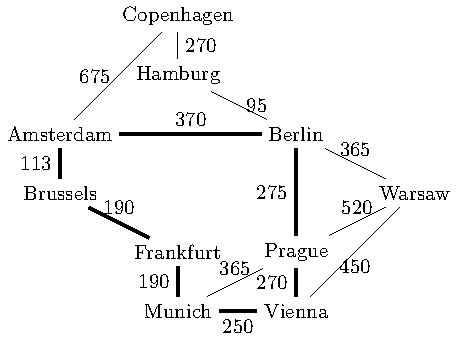
\includegraphics[width=\linewidth]{not_hamiltonian}
  \caption{{\color{red}\ding{55}} Not a Hamiltonian cycle.}
  \end{subfigure}
  \begin{subfigure}[t]{0.32\linewidth}
  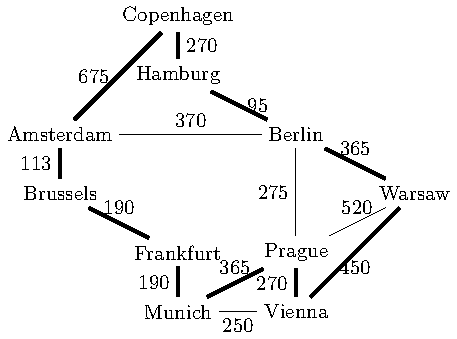
\includegraphics[width=\linewidth]{not_shortest}
  \caption{{\color{red}\ding{55}} Not the shortest Hamiltonian cycle. (Length: $3028$ Minutes)}
  \end{subfigure}
  \begin{subfigure}[t]{0.32\linewidth}
  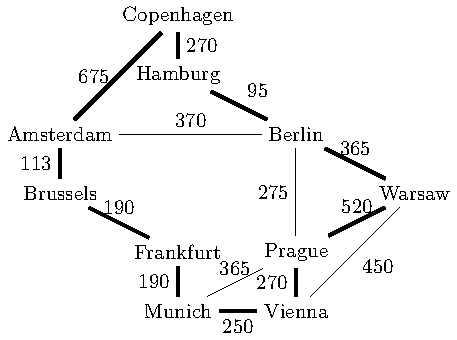
\includegraphics[width=\linewidth]{shortest}
  \caption{{\color{green}\ding{51}} Solution to the TSP. (Length: $2938$ Minutes)}
  \end{subfigure}
  \end{figure}
  \end{center}
  \item The best general classical algorithms take exponential time in $n$.
  \end{itemize}
  \end{block}

  \begin{block}{\Large 2. Backtracking algorithms}
  \begin{itemize}
  \item Backtracking algorithms are a way of solving constraint satisfaction problems.
  
  \item They have two parts:
  \begin{enumerate}
  \item A predicate, which checks if the constraints are satisfiable;
  \item and a heuristic, which chooses the next variable to assign.
\end{enumerate}

  \item When called with a partial assignment, the predicate checks if the constraints are satisfiable. If not, we return.
  
  \item Otherwise, the heuristic picks a variable which we assign a value to and recursively call ourselves with this new partial assignment.
  
  \item Montanaro [Mon15] developed a quantum backtracking algorithm which has a quadratic speedup for finding a solution.
  \end{itemize}
  \end{block}

  \begin{block}{\Large 3. Quantum speedup for degree-3 graphs}
  \begin{itemize}
  \item Backtracking algorithms can solve the TSP with ``forced'' edges which me must travel down and ``removed'' edges which we must avoid travelling on.
  
  \item The predicate checks if a Hamiltonian cycle is possible, and the heuristic selects another edge to force or remove.

  \item The best backtracking algorithm on degree-3 graphs runs in {\color{uobred} $O^*(2^{3n/10})$} time and polynomial space [XN16a].
  
  \item We apply [Mon15] to this algorithm to find a Hamiltonian cycle, failing to find one when one exists with probability $\delta$, in {\color{uobred}$O^*(2^{3n/20}\log(1/\delta))$} time, where $O^*$ hides polynomial factors.
  
  \item We find the shortest Hamiltonian cycle with bounded error (finding a sub-optimal cycle or no cycle) via binary search with {\color{uobred}$O(\log L\log\log L)$} overhead, where $L$ is the longest edge length.
  \end{itemize}
  \end{block}
  \end{column}

  \begin{column}{0.422\linewidth}
  
  \begin{block}{4. Example backtracking step}
  \begin{figure}
  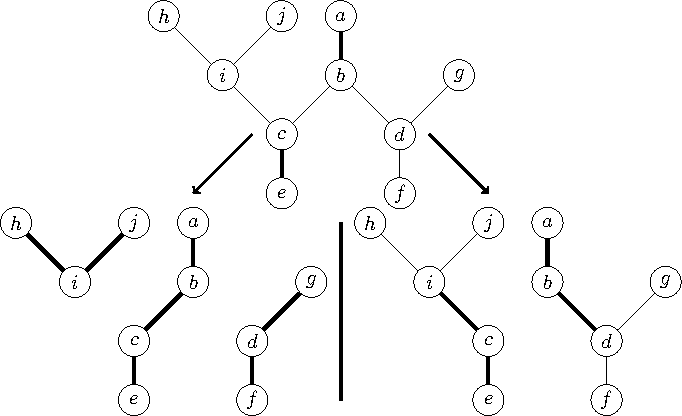
\includegraphics[width=\linewidth]{reduction}
  \end{figure}
  \begin{itemize}
  \item Forcing $bc$, as shown on the left, means that $b$ and $c$ are incident to two forced edges, so $ci$ and $bd$ are removed. Now $d$ and $i$ are of degree 2, so edges $df, dg, hi$ and $ij$ are forced.
  
  \item Removing $bc$, as shown on the right, means that $b$ and $c$ are of degree 2, so edges $bd$ and $ci$ are now forced.
  \end{itemize}
  \end{block}

  \begin{block}{\Large 5. Expanding to higher-degree graphs}
  \begin{figure}
  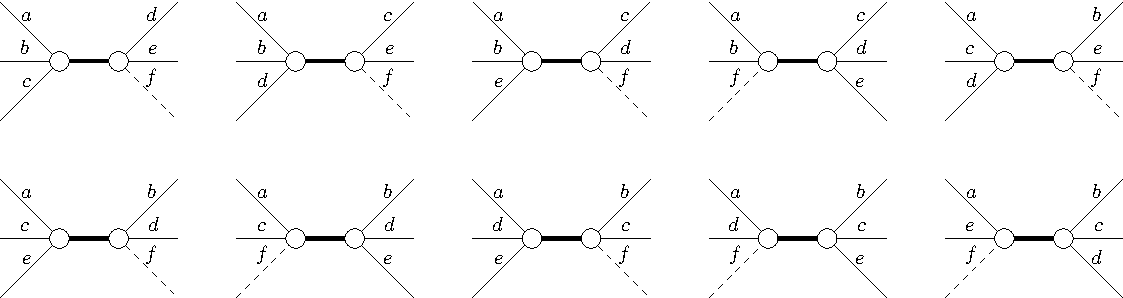
\includegraphics[width=\linewidth]{deg5}
  \caption{Ways of splitting a vertex of degree 5 or 6 into two lower-degree vertices.}
  \end{figure}

  \begin{itemize}
  \item For degree-4 graphs, we apply the same technique to the algorithm of [XN16b] in {\color{uobred}$O^*(1.301^n\log L \log\log L)$} time.
  
  \item Other speedups can be found by breaking higher-degree vertices into degree 4 vertices connected by forced edges.
  
  \item We find the shortest way of splitting each vertex via [DH99].

  \item For degree-5/6 graphs, there are 10 ways of splitting each vertex, of which 6 will preserve the shortest Hamiltonian cycle. Thus we get an additional {\color{uobred} $O((10/6)^{n/2})$} overhead.

  \item For degree-7 graphs, this method is slower than classical algorithms for the general TSP [HK62, Bj\"o14].
  \end{itemize}
  \end{block}

  \begin{block}{\Large References}
  [Bj\"o14] A. Bj{\"o}rklund, SIAM Journal on Computing, 43(1):280--299 (2014)

  \noindent[DH99] C. D\"urr and P. H\o yer, {\tt arXiv:quant-ph/9607014} (1999)

  \noindent[HK62] M. Held and R. Karp, Journal of the Society for Industrial and Applied Mathematics, 10(1):196--210, (1962)

  \noindent[Mon15] A. Montanaro, {\tt arXiv:1509.02374} (2015)

  \noindent[XN16a] M. Xiao and H. Nagamochi, Algorithmica 74(2):713--741, (2016)

  \noindent[XN16b] M. Xiao and H. Nagamochi, Theory of Computing Systems, 58(2):241--272, (2016)
  \end{block}
  \end{column}
\end{columns}

\end{frame}

% -----------------------------------------------------------------------------

\end{document}



